\documentclass[german,version-2020-11]{uzl-thesis}


% Copy this file as a template for your thesis. You will have to take
% action at all places marked by
%
% !!!!!!!!!!!!!!!!!!!!!!!!!!!!!!!!!!
% !!! Your action is needed here !!!
% !!!!!!!!!!!!!!!!!!!!!!!!!!!!!!!!!!
%
% The first place your action is needed is the first line of this
% document:
%
%
% Language of the thesis:
%
% You must use either 'german' or 'english' above, depending on the
% language used in the main text. This will automatically setup a lot
% of things in the background.
%
%
% Version of the class:
%
% You must specify which version of the thesis class is to be
% used. This is important in case the class style changes in later
% years, but we still want an older thesis to look the same, even when
% things are changed in the class.
%
% Do not change or remove the version-xxxx key.
%
%
% Text encoding:
%
% Your thesis *must* be encoded in utf8 (unicode), which is the
% default in most editors these days. Do *not* change this to latin8.



%%%
%
% Main setup:
%
%%%
%
% You must use the \UzLThesisSetup command to specify numerous things
% about your thesis. This includes the entries on the title page, the 
% abstracts, and the bibliography style. You do so by specifying
% so-called "values" for so-called "keys". For instance, 
% for the key "Autor" you must provide your name as the value. You do
% so by writing 'Autor = {Max Mustermann}', that is, the value is put
% into curly braces. You can use the \UzLThesisSetup command
% repeatedly and the order in which you provide the keys is not
% important. 
%
% Everything shown on the title page must be in German -- even
% if the thesis is written in English! Just insert German text for
% German keys and English text for English keys (like 'Abstract' needs
% English text, while 'Zusammenfassung' needs German text).

\UzLThesisSetup{
  %
  % !!!!!!!!!!!!!!!!!!!!!!!!!!!!!!!!!!
  % !!! Your action is needed here !!!
  % !!!!!!!!!!!!!!!!!!!!!!!!!!!!!!!!!!
  %
  % First, specify the institut or clinic at which the thesis was
  % written. You get the logo file from them (make sure it has the
  % correct size, namely the same as the example). If they do not have
  % a logo, the university's default logo is used.
  %
  % The 'verfasst' gets two arguments. Change the first to {an der}
  % for clinics, as in 'Verfasst = {an der}{Medizinischen Klinik I}'
  %
  Logo-Dateiname        = {uzl-thesis-logo-itcs.pdf},
  Verfasst              = {am}{Institut für Theoretische Informatik},
  %
  % The titles:
  %
  Titel auf Deutsch     = {
    Vorlage für die \LaTeX-Klasse »uzl-thesis« zur Nutzung bei
    Bachelor-~und Masterarbeiten an der  Universität~zu~Lübeck
  }, 
  Titel auf Englisch    = {
    Template for the \LaTeX\ Class “uzl-thesis” for
    Bachelor's and Master's Theses Written at the University~of~Lübeck 
  },
  %
  % Author and supervisor:
  % 
  % Note that the 'Betreuer' or 'Betreuerin' is the supervisor, that
  % is, the professor who officially supervises the thesis. If there
  % is also an assistent of the professor who helped (typically a
  % lot), use 'Mit Unterstützung von' to thank that person. If the
  % thesis was mainly written 'externally' at some company or another
  % institute, point this out using 'Weitere Unterstützung'. 
  % 
  % For your own name, do *not* add things like "BSc" or "BSc
  % cand.". For the supervisor, you should normally include
  % "Prof. Dr." or "PD Dr." (ask your supervisor, what is
  % appropriate), but nothing more (so no
  % "Univ.-Prof. Dr. Dr. h.c. mult." unless your supervisor insists).  
  %
  Autor                 = {Leonard },
  Betreuerin            = {X},
  % 
  % Optional: Supporting persons and institutions. The text should be
  % in German, even for an English thesis.
  %
  Mit Unterstützung von = {Harry Hilfreich},
  % 
  %   Weitere Unterstützung = {
  %     Die Arbeit ist im Rahmen einer Tätigkeit bei der Firma Muster GmbH
  %     entstanden.
  %   },
  %
  %
  % Your Degree Programm (Studiengang)
  %
  % Specify 'Bachelorarbeit' or 'Masterarbeit' and the degree
  % programme. Make sure the name of programme is correct and not
  % some abbreviation or some incorrect variant. For instance:
  % 'Medizinische Ingenierwissenschaft', but not 'MIW';
  % 'Medizinische Informatik', but not 'Medizin-Informatik';
  % 'Informatik', but not 'Informatik (SSE)'.
  %
  % Use German names for German programmes and English names for
  % English ones, so 'Infection Biology', not 'Infektionsbiologie'. 
  % For programmes that have a German bachelor and an English master,
  % use the German name for a bachelor thesis and the English name for
  % the master thesis.
  %
  Bachelorarbeit,
  Studiengang           = {Informatik},
  %
  % Date on which the thesis is turned in German, formatted the
  % traditional German way:
  %
  Datum                 = {1. Januar 2021},
  %
  % The English abstract. You must always provide abstracts in German
  % and in English. 
  %
  Abstract              = {
    It is not easy to write a thesis that does not only advance
    science, but that is also a pleasure to read. While the scientific
    contribution of a thesis is undoubtedly of greater importance, the
    impact of \emph{writing well} should not be underestimated: If
    the person who grades a thesis finds no pleasure in the reading,
    that person are also unlikely to find pleasure in giving outstanding
    grades. A well-written text uses good German or English phrasing with a clear and correct 
    sentence structure and language rhythm, there are no spelling
    mistakes and the author's arguments are presented in a
    clear, logical and understandable manner using well-chosen
    examples and explanations. In addition, a nice-to-read font and a
    pleasing layout are also helpful. The \LaTeX\ class presented in
    this document helps with the latter: It contains a number of
    ready-to-use designs and 
    takes care of many small typographical chores.
  },
  Zusammenfassung       = {
    Es ist nicht leicht, eine Abschlussarbeit so zu schreiben, dass sie
    nicht nur inhaltlich gut ist, sondern es auch eine Freude ist, sie
    zu lesen. Diese Freude ist aber wichtig: Wenn die Person, die die 
    Arbeit benoten soll, wenig Gefallen am Lesen der Arbeit findet,
    so wird sie auch wenig Gefallen an einer guten Note
    finden. Glücklicherweise gibt es einige Kniffe, gut lesbare
    Arbeiten zu schreiben. Am wichtigsten ist zweifelsohne, dass
    die Arbeit in gutem Deutsch oder Englisch verfasst wurde mit klarem
    Satzbau und gutem Sprachrhythmus, dass keine Rechtschreib- oder
    Grammatikfehlern im Text auftauchen und dass die Argumente der
    Autorin oder des Autors klar, logisch, verständlich und gut
    veranschaulicht dargestellt werden. Daneben sind aber auch gut
    lesbare Schriftbilder und ein angenehmes Layout hilfreich. Die Nutzung
    dieser \LaTeX-Vorlage hilft der Schreiberin oder dem Schreiber
    dabei zumindest bei Letzterem: Sie umfasst gute, sofort nutzbare
    Designs und sie kümmert sich um viele typographische
    Details.  
  },
  %
  % Optional: 'Danksagungen' (German) or 'Acknowledgements'
  % (English). Both keys are optional and both have the same effect of
  % adding an acknowledgements text after the abstracts and before the
  % table of contents.
  %
  Acknowledgements      = {
    This is the place where you can thank people and institutions, do
    not try to do this on the title page. The only exception is in
    case you wrote your thesis while working or staying at a company or abroad. Then you
    should use the \Latex{Weitere Unterstützung} key to provide a text
    (in German) that acknowledges the company or foreign
    institute. For instance, you could use texts like »Die Arbeit
      ist im Rahmen einer Tätigkeit bei der Firma Muster GmbH
      entstanden« or »Die Arbeit ist im Rahmen eines
      Forschungsaufenthalts beim Institut für Dieses und Jenes an der
      Universität Entenhausen entstanden«. Do not name and thank
      individual persons from the company or foreign institute on the
      title page, do that here. 
  },
  % Bibliography style: Choose between
  % 
  % 'Alphabetische Bibliographie'
  % for all degree programmes in the natural sciences 
  % 
  % 'Numerische Bibliographie'
  % alternative for all other degree programmes
  % 
  % Either will load biblatex and setup the citation methods and the
  % bibliography styles correctly. You should not mess with them.
  % 
  Alphabetische Bibliographie,
  % Alternatively:
  % Numerische Bibliographie
}




%%%%%%%%%%%%%%%%%%%%
%
% Styling the thesis
%
%%%%%%%%%%%%%%%%%%%%
%
% Creating a visually pleasing layout and choosing fonts is not
% easy. Furthermore, different people have different preferences. Of
% course, for the University of Lübeck, the dean of studies could just
% force everyone to use one specific layout and font, but that seems a
% bit drastic and, also, it seems nice that thesis by different people
% have an individual style even though they all stick to the same
% overall structure.
%
% For these reasons, I (Till Tantau) have spend quite some time on
% designing a flexible layout and styling mechanism for theses.
%
% Basically, the overall structure of the thesis is fixed by the
% thesis class and so are many structural elements. For instance, you
% cannot change the order in which the abstract and table of contents
% are shown, you cannot move the bibliography elsewhere, indeed, the
% bibliography style is also fixed. Likewise, the text on the title
% page is fixed.
%
% Although many things are fixed, you *can* change several other
% things. For instance, you can change the font used for the main
% text, you can change which font is used for titles and headings or
% you can change whether titles and headlines are centered or flushed
% left.
%
% There are many LaTeX packages for changing such things. You are
% kindly asked *not to use them*. Rather, use (only) the options
% offered by the thesis class. All possible choices and combinations
% there have been tested by me and produce nice results; what happens
% with other packages no one knows and might no longer conform to what
% is expected by the university. As you will see, you still have a
% lot of options.
%
%
% Technical note: All styling is done via the command
%
% \UzLStyle{...}
%
% where ... is a key-value list just as for \UzLThesisSetup. The
% difference is just that everything having to do with styling as
% controlled by \UzLStyle, while the more “formal” setup keys are
% controlled by \UzLThesisSetup.
%
%%%
%
% Designs
%
%
% A \emph{design} is a whole set of font and layout options bundled
% together. They have been chosen in such a way that a visually
% pleasing “overall appearance” results.
%
%
% \UzLStyle{computer modern oldschool design}
%
% The look of this design mimics the “classical” way a paper or report
% created with \LaTeX\ looks like: The Computer Modern font is used,
% bold face fonts are used for headlines, only black and white are
% used as colors. This design reminds me of older scientific
% documents, especially from the computer science community where
% \LaTeX\ was used very early.
%
%
% \UzLStyle{computer modern basic design}
%
% A slightly less “oldschool” version of the previous design. It is
% still a classic design in the sense that it uses the Computer Modern
% font and that it still has this “good old \LaTeX” look, but some
% more modern aspects (like colors!) have been added.
%
% Note that this design uses Myriad for the title page (one of the
% “modern aspect”), which means that his font must be installed.
%
%
% \UzLStyle{computer modern scholary design}
%
% In my opinion, this is the ultimate “scholary design”: The thesis
% will look like it has been typeset by hand some 150 years ago and
% then printed by a university press. There is really nothing “modern”
% about it and the word in the name of the design is just part of the
% name of the “Computer Modern” font.
%
%
% \UzLStyle{pagella basic design}
%
% A, well, basic design that uses the Pagella font rather than the
% Computer Modern font. Especially the bold face version of this font
% looks nicer than the Computer Modern counterpart. Also, Pagella,
% while still having a “bookish” look, still feels a bit fresher than
% Computer Modern. 
%
%
% \UzLStyle{pagella centered design}
%
% A variant of the basic Pagella design that centers all
% headlines. A nice alternative to the basic version.
%
%
% \UzLStyle{pagella contrast design}
%
% This design tries to create some visual friction by contrasting the
% sans serif headline font (in bold!) with the main text. I find it a
% visually very interesting combination.
%
%
% \UzLStyle{alegrya basic design}
%
% The third variant of the basic design, this time using the Alegrya
% font. 
%
%
% \UzLStyle{alegrya scholary design}
%
% The Alegrya version of the previous “scholary” design. Unlike the
% Computer Modern version, this design does not look old, but more
% fresh -- while still creating the impression that the text must be
% about a very scientific subject. 
%
%
% \UzLStyle{alegrya stylish design}
%
% The design is quite similar to the scholary version for the Alegrya
% font, but with even more modern additions. “Stylish” is the word
% that comes to my mind.
%
%
\UzLStyle{alegrya modern design}
%
% A design that uses the sans serif version of the Alegrya font for
% the headlines. This is a nice modern overall design.
%
%%%




%%%%%%%%
%
% Now, include the package you need here using \usepackage. 
%
% However, many standard packages are already loaded by the class:
%
% amsmath, amssymb, amsthm, babel, biblatex, csquotes, etoolbox,
% filecontents, fontspec, geometry, hyperref, tikz (with libraries
% arrows.meta, positioning and shapes), varioref, url 
%
% Indeed, in many cases you will not need any extra packages.
%
%%%%%%%


\usepackage{graphicx}
\usepackage{listings}
\usepackage{xcolor}
\usepackage{comment}
\usepackage{tikz}
\usepackage{amsmath}
\usetikzlibrary{arrows, automata, positioning}


\begin{document}

%
% The title page and table of contents will be inserted automatically
% here. 
%


\chapter{Einleitung}
% In a German thesis write: \chapter{Einleitung}


% !!!!!!!!!!!!!!!!!!!!!!!!!!!!!!!!!!
% !!! Your action is needed here !!!
% !!!!!!!!!!!!!!!!!!!!!!!!!!!!!!!!!!
%
% Replace with your own introduction:

% DELETE the following line for your own thesis - it causes trouble!
\lstMakeShortInline[style=code,style=inline,language={[LaTeX]tex},moretexcs={chapter}]|



\section{Contributions of this Thesis}



\section{Related Work}


\section{Structure of this Thesis}

\chapter{Hauptteil}
\section{Motivation}
Die digitalisierte Welt generiert täglich riesige Mengen an neuen Informationen. Die Kapazitäten, die ein Mensch aufbringen kann, um solche Massen an Daten zu organisieren und zu verstehen, sind schon lange übertroffen. Topic Modeling (dt. Themenmodellierung) beschreibt eine Gruppe von Verfahren, die es ermöglichen, große elektronische Datensammlungen automatisiert zu durchsuchen, organisieren und zu verstehen. Es können Muster innerhalb der Daten entdeckt und Themen extrahiert werden. Dabei stellen Themenmodelle statistische Modelle dar, die Verwendung in der Inferenz abstrakter Themen in unsortierten Datenmengen finden. In einer Welt von exponentiell wachsenden Datenmengen finden Methoden der Themenmodellierung stetig eine breitere Anwendung. Bereits heute wird Themenmodellierung in vielen Bereichen der Wirtschaft, Wissenschaft und Informationstechnologie verwendet. Um semantische Folgerungen aus Datenmengen zu generieren, gibt es verschiedene Ansätze – in dieser Arbeit wird es um die ‚Latent Dirichlet Allocation‘ gehen. Dabei werden ähnliche Wörter, die in ähnlichen Kontexten vorkommen in einem Cluster gruppiert. 

\section{Ziel}
Diese Arbeit wird die Theorie der Themenmodellierung anhand des Beispiels des Zweckverband Ostholstein (ZVO) implementieren und die bezüglichen Parameter im Sinne der Auswertung bewerten. Der ZVO erhält jährlich ein große Menge an Kundenanfrage. Diese werden momentan händisch an die jeweils zuständige Abteilung weitergeleitet. Der Prozess soll zukünftig automatisch durch einen Klassifikationsmechanismus funktionieren. Nach der Implementation eines LDA Algorithmus zur Inferenz verschiedener Abteilungen aus den Kundenanfragen, kann die momentan händische Kategorisierung bewertet werden. Diese Arbeit beschäftigt sich mit der Vorhersage der Qualität des Klassifikators, indem die Qualität der manuell erstellten Kategorien und Kundenanfrage-Gruppen untersucht und mit den Ergebnissen verschiedener Themenmodellierung verglichen wird. Das Ergebnis einer Themenmodellierung hängt stark von der Qualität der Daten ab, die sie als Input bekommt. Diese Daten durchlaufen eine Reinigungsphase, bevor sie klassifiziert werden, um sie in eine gut zu verarbeitende Form zu bringen. 

\section{Notation}

\begin{itemize}
	\item $\mathcal{K}$ ist die Anzahl der Themen in einem Topic-Modell $\mathcal{M}$
	\item Ein Model $\mathcal{M}$ repräsentiert den Korpus $\mathcal{D}$
	\item Eine Menge von Dokumenten ist ein Korpus $\mathcal{D}$
	\item Ein Dokument $\mathcal{d}$ eines Korpus ist eine Menge von $\mathcal{N}$-vielen 
	Worten 
\end{itemize}


\section{Modellvergleich}
\subsection{Latent Dirichlet Allocation}
Themenmodellierung besteht aus vielen Methoden, die meist verbreitete ist die „Latent Dirichlet Allocation (LDA)“, was als Bag of Word modelliert ist, also keine Kontextinformationen beinhaltet. Dieses Verfahren ist eine Weiterentwicklung des ‚PLSI‘, das durch zwei Dirichlet-Priors ergänzt wurde. LDA liegt ein generierender Prozess zugrunde, den zwei Dirichlet Verteilungen maßgeblich beeinflussen: die Dokument-Themen Verteilung, die die Ausprägungen verschiedener Themen in einem Dokument beschreibt, und die Themen-Wörter Verteilung, die die Wahrscheinlichkeit beschreibt, dass ein bestimmtes Wort in einer gewissen Regularität in einem Themenbereich vorkommt. Dabei geht man davon aus, dass ein Dokument eine Verteilung von Themen ist, während ein Thema als eine Verteilung über Wörter betrachtet wird. 
Die Wahrscheinlichkeit, dass ein bestimmtes Dokument generiert wird, ist das Produkt der Wahrscheinlichkeiten der beiden Verteilungen mit den Wahrscheinlichkeiten zweier multinomialen Verteilungen, die erst zufällig Topics, wie in der Dirichlet-Verteilung definiert, auswählen und aus diesen dann, mithilfe der zweiten Dirichlet-Verteilung, Wörter aus diesen Topics herleiten, wodurch das Enddokument entsteht. Das Enddokument wird höchstwahrscheinlich stark von dem gegebenen Dokument abweichen, jedoch kann durch anpassen der Dirichlet-Verteilungen ein Optimierungsproblem formuliert werden, nach dem die Dirchlet-Verteilungen gesucht werden, die ein möglichst ähnliches Dokument generieren.

\subsection{Latent Semantic Analysis (LSA)}
Ein anderes verbreitetes Verfahren ist das „Latent Semantic Analysis“ (LSA), welches auf das Finden von sogenannten Hauptkomponenten in Dokumenten abzielt. Dadurch können sowohl ähnliche Wörter gefunden, als auch Textbereiche, die inhaltliche Überschneidungen mit einem bestimmten Begriff haben, aber das Wort selber nicht enthalten, gefunden werden. Die Methode basiert auf dem Prinzip der Singulärwertzerlegung(SVD). Als Ausgangslage wird aus einer Textsammlung eine Term-Dokument-Matrix erstellt. Diese Matrix wird in der SVD als Produkt von drei Matrizen dargestellt, von denen die mittlere eine Diagonalmatrix darstellt. Die Werte auf der Diagonalen lassen daraus die Topics der Textmenge ablesen. Auf das SVD Verfahren selbst hat der Entwickler wenig Einfluss. Um Rauschen zu verhindern, kann jedoch die Anfangsmatrix mithilfe der term-frequency und inverse-document-frequency verbessert werden, was sich auf das Gesamtergebnis auswirkt. LSA stellt sich als ein attraktives Verfahren heraus, da es Synonyme besser erkennen kann, als LDA und wird heutzutage unter anderem intensiv in dem Bereich des Digital Marketings genutzt.

\subsection{Non-Negative Matrix Factorization (NMF)}
Ein weiteres Verfahren, das auch mit Matrizen funktioniert, wird „Non-Negative Matrix Factorization“ (NMF) genannt. Dabei wird eine Matrix, die Wörter auf Dokumente abbildet, in zwei Teilmatrizen faktorisiert. Die erste Teilmatrix stellt die Topics in Dokumenten, die zweite die Wörter in Topics dar. Dadurch kann Speicherplatz gespart, und Themen aufgedeckt werden. Das Verfahren beginnt mit zwei möglichen faktorisierten Matrizen und verbessert sich durch die Errorfunktion iterativ, bis das Ergebnis gut genug ist. Dabei werden die errechneten Werte mit der gegebenen Matrix verglichen und angepasst.


\section{Grundlagen der Latent Dirichlet Allocation (LDA)}
Latent Dirichlet Allocation ist ein grundlegendes und bekanntes Verfahren aus der Natürlichen Sprachverarbeitung. Das Prinzip der Themenmodellierung basiert auf einer Menge an Dokumenten, die den Korpus darstellen. Dabei werden alle Dokumente als Menge von Wörtern angenommen, die als Bag of Words modelliert sind. Dabei hat weder die Reihenfolge, noch die Groß- und Kleinschreibung Einfluss auf das Ergebnis. Die Themen werden  allein an der Vorkommenswahrscheinlichkeit der Wörter ohne Reihenfolgen- oder Kontextinformationen erkannt. Durch die Reduktion der Dimension wird die Effizienz gesteigert. Somit wird also jedes Dokument durch eine Verteilung der enthaltenen Wörter repräsentiert.\\

Eine Besonderheit bei der Themenerkennung mit LDA ist, dass die Anzahl der gesuchten Themen \mathcal{K} vorgegeben werden muss. Oft ist diese vorher jedoch nicht bekannt und muss über Hilfsverfahren, wie der Perplexitätsberechnung ermittelt werden. Die Funktionsweise von LDA ist über folgende graphische Abbildung beschrieben: \\

\begin{center}
\begin{tikzpicture}
	\draw (0,0) [very thick] rectangle (9,3) 
	\draw [very thick](6,3.5) rectangle (9,5.5)
	\draw [very thick](3,0.25) rectangle (8.75,2.75)
	\draw (1.5,1.5) circle [very thick, radius = 0.8]  node {$\theta$};
	\draw (4.5,1.5)  circle [very thick, radius = 0.8] node {$\mathcal{Z}$};
	\draw (7.5,1.5) circle [fill=black, ultra thick, radius = 0.8, accepting] node {$W$};
	\draw (-1.5,1.5) circle [very thick, radius = 0.8] node {$\alpha$};
	\draw (7.5,4.5) circle  [very thick, radius = 0.8] node {$\beta$};
	\draw (4.5,4.5) circle  [very thick, radius = 0.8] node {$\phi$};
	
	\draw [->,ultra thick] (5.3,4.5) -- (6.7,4.5)
	\draw [->,ultra thick] (7.5,3.7) -- (7.5,2.3)
	\draw [->,ultra thick] (5.3,1.5) -- (6.7,1.5)
	\draw [->,ultra thick] (2.3,1.5) -- (3.7,1.5)
	\draw [->,ultra thick] (-0.7,1.5) -- (0.7,1.5)
	
\end{tikzpicture}   
\end{center}\\

Dabei beschreibt \mathcal{W} als einzige nicht verborgene Variable eines von \mathcal{N} Wörtern des Dokuments. Das Wort ist semantisch einem Thema \mathcal{Z} zugeordnet. Das Thema wiederum hängt von der Themen-Verteilung \mathcal{theta} des Dokuments ab, das als ein Elment der \mathcal{M} vorliegenden Dokumente betrachtet wird. Neben dem Thema, wird jedes Wort auch von der jeweilgen Thema-Wort-Verteilung \mathcal{\phi} der \mathcal{K} Themen beeinflusst. Das Modell und dessen Verteilungen kann durch die Parameter $\alpha$ und $\beta$ angepasst werden. $\alpha$ kann bestimmt die Intensität der Dokument-Themen-Verteilung, während $\beta$ die der Themen-Wort-Verteilung beeinflusst. Bei einem großen $\alpha$ ist die Verteilung der Themen in einem Dokument ähnlicher. Zusätzlich werden bei LDA zwei Bedingungen verfolgt, die von den beiden Parametern beeinflusst werden können. Erstens strebt man für alle Wort eines bestimmten Dokuments so wenig zugeordnete Themen an, wie möglich. Zweitens soll ein Thema über so wenig relevante Wörter wie möglich verfügen. Die beiden Ziele stehen in einer Wechselbeziehung zueinander, da eine minimale Anzahl an vertretenen Themen in einem Dokument zu maximal vielen Wörtern in diesen Themen führt. Die minimale Anzahl an Themen wäre erreicht, wenn man alle Wörter eines Dokuments einem Thema zuweist. Dadurch verfügt das Thema jedoch über alle Wörter des Dokuments. $\alpha$ befindet sich in dem Bereicht $[0,1]$ mit sinnvollen Werten zwischen $[0.01, 0.1]$, während $\beta =0.01$ durchschnittlich die besten Ergebnisse liefert. Große Werte führen zu einer Gleichverteilung, die wiederum eine Verschlechterung der Perplexität bedeutet. Somit bietet die Perplexität ein Mittel, um $\alpha$ und $\beta$ optimal für die individuelle Anwendung zu finden. \\

Bei LDA werden zwei Verteilungen aus den Dokumenten $d \in \mathcal{D}$ und $k \in \mathcal{K}$gelernt: die Dokument-Topic-Verteilung $\theta$ und die Topic-Wort-Verteilung $\phi$. Dabei gibt die Dokument-Topic-Verteilung an, mit welcher Wahrscheinlichkeit das Dokument zu jedem Themen gehört. Die Topic-Wort-Verteilung berechnet die Wahrscheinlichkeit, dass ein Wort einem Thema angehört. $\mathcal{M} = LDA(\mathcal{D})$ beschreibt ein LDA Modell, das auf der Dokumentenmenge/Korpus $\mathcal{D}$ trainiert wurde.


\subsection{Der generative Prozess} 
Der Algorithmus hinter LDA generiert neue Dokumente mithilfe von Dirichletverteilungen $Dir(\gamma)$ und Multinomialverteilungen $Multinom(\delta)$. Die Verteilungen $\theta$ und $\phi$ werden errechnet, indem iterativ neue Dokumente über andere Verteilung generiert werden, bis das generierte Dokument die Anforderungen befriedigt, dann können die Verteilungen abgelesen werden, mit denen das Dokument erstellt wurde. Der Prozess verläuft folgendermaßen: 
\begin{enumerate}
	\item Wähle ein $\theta$ als $Dir(\alpha)$
	\item Wähle ein $\phi$ als $Dir(\beta)$
	\item Für jedes Wort $w$ and Stelle $i = 1,...,N$ im Dokument $d$: 
	\begin{enumerate}
		\item Wähle ein Thema $z_{d,i}$ als $Multinom(\theta_d)$
		\item Wähle ein Wort $w_{d,i}$ als $Multinom(\phi_z_{d,i})$
	\end{enumerate}
\end{enumerate}

Somit kann der Algorithmus nun neue Dokumente erstellen und das Ergebnis durch die Parameter, wie Alpha und Beta, anpassen, bis das Ergebnis ähnlich genug zu dem Anfangsdokument ist. Dann ist die Verteilung der Themen in diesem Dokument bekannt. Bei der Anwendung von LDA für praktische Problemstellungen, geht LDA das Prinzip rückwärts durch, d.h. für bestehende Gruppen an Dokumenten werden Verteilungen gesucht, durch die das Dokument generiert hätte werden können.

\begin{equation}
P(w,z,\theta, \phi, \alpha, \beta) = \bigg{\prod} P(\theta, \alpha) \cdot \prod P(\alpha, \beta) \cdot \prod P(z,\tehta) \cdot \prod P(w \mid \phi) 
\end{equation}

Die Formel beschreibt die totale Wahrscheinlichkeit des LDA Modells. Sie setzt sich zusammen aus den Produkten der Dirichlet Verteilung der Topics und der Wörter zusammen mit den multinomialen Verteilungen der Themen und Wörter. Die Schwierigkeit des Algorithmus besteht in der Berechnung der $\theta$-Verteilung der gegebenen Dokumente für latente Variablen. Dies lässt sich durch folgende Wahrscheinlichkeitsverteilung ausdrücken: 

\begin{center}
\begin{equation}
P(\theta, z \mid w, \alpha, \beta) = \frac{P(\theta, z, w \mid \alpha, \beta)}{P(w \mid \alpha, \beta)}
\end{equation}
\end{center}

Die Formel berechnet die Wahrscheinlichkeit der Verteilung unter einem bestimmten Thema gegeben der $\alpha$ und $\beta$ Parameter und dem bekannten Wort. Die Wahrscheinlichkeit kann nicht exakt bestimmt werden, weshalb Verfahren wie Gibbs Sampling diese approximieren.


%\begin{center}
%\includegraphics{img1.png}
%\end{center}


\section{Daten}
Die Daten liegen in folgendem Format vor: 

\begin{center}
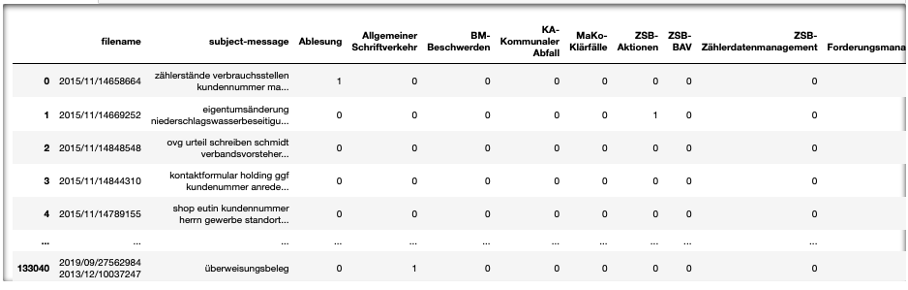
\includegraphics{daten1}
\end{center}

Relevant für die Auswertung sind die subject-message und die jeweilige Abteilung. Die Tabelle verfügt über eine Matrix mit 18 Abteilungen, von denen pro subject-message eine mit einer 1 versehen ist. Dies beschreibt die Abteilung, der diese Anfrage manuell zugeordnet wurde. Die Daten in subject-message sind bereits bereinigt, also liegen vor, wie in diesem Beispiel, der Zeile 0:

\begin{center}
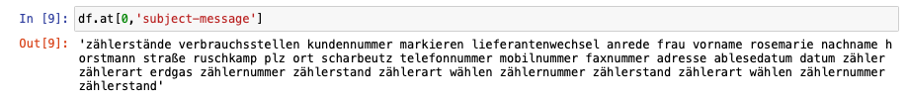
\includegraphics{daten2}
\end{center}

Um die Einträge in eine computer-lesbare Form zu verwandeln, muss ein Dictionary erstellt werden, dass alle Wörter auf eine Anzahl ihrer Vorkommen abbildet. Dafür müssen die Wörter als alleinige Listeneinträge einlesbar sein: 

\begin{center}
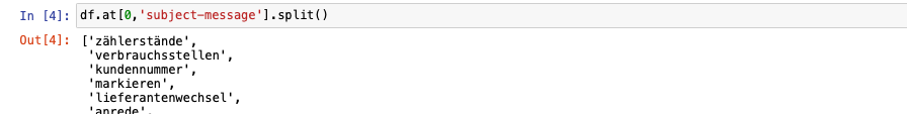
\includegraphics{daten3}
\end{center}

\subsection{Gibbs Sampling}
\subsection{Hellinger Distanz}

\subsection{Datenreinigung}
Bevor eine Themenmodellierung auf Daten durchgeführt werden kann, müssen die Daten einem Prozess unterzogen werden. Dieser beginnt mit der Datenaquise, also der Akquirierung bestimmter relevanter Daten. Im Falle der ZVO bedeutet dies, dass es genügend Kundenanfragen gibt, die verarbeitet werden können. Wenn diese Daten bestehen, werden sie auf die relevanten Wörter reduziert, aus denen eine bedeutsame Inferenz von Informationen möglich ist, sodass unter anderem die sogeneannten „Stop-Words“, also eine Menge von Verbindungswörtern entfernt werden. Ein anderer Schritt der Datenreinigung ist das Transponieren aller Wörter in kleine Buchstaben, um eine Einheitlichkeit zu erlangen, da das Bag of Words Modell keine Reihenfolge mehr beachtet und somit große Satzanfänge irrelevant werden. Wenn die Daten in der gewünschten Form vorliegen, beginnt der Schritt des Featureengineerings. Für einen Computer sind Wörter nicht so leicht zu verarbeiten, wie Zahlen, weshalb in diesem Schritt eine Quantisierung der Wörter und Überführung dieser in eine zahlenbasierte Form vorgenommen wird. Dies kann zum Beispiel in Form eines Bag-of-Words Modells, Dictionary oder TF-IDF, also einer relativen Vorkommensauflistung verschiedner Wörter über Dokumente umgesetzt werden. Nachdem die Daten in eine für den Computer kompatiblen Form gebracht wurden, kann das Themenmodell entwickelt werden. 

\section{Ansätze}
In diesem Abschnitt werden verschiedene Möglichkeiten implementiert und analysiert, wie LDA im Sinne der ZVO genutzt werden kann. Dabei ist die Zielfrage, wie am besten für ein unbekanntes Dokument die bestimmte Abteilung gefunden werden kann. Dafür müssen Korpora bestehen, die bereits durch Verteilung definiert sind, sodass die Dokument-Themen Verteilung für das neues Dokument inferiert werden kann. Wenn die Themenverteilung des neuen Dokuments gegeben ist, kann über Vergleiche der Verteilungen mit Dokumenten oder Durschnitten von Korpora eine Abteilung für das Dokument identifiziert werden. 

Die Möglichkeiten, die sich für diesen Zweck ergeben sind folgende: 
\begin{enumerate}
\item Alle Dokumente ergeben ein Korpus. Das neue Dokument wird mit dem gesamten Korpus verglichen und auf thematische Kompatibilität geprüft. Ein Gesamtbild der thematischen Aufteilung aller Dokumente kann eine mögliche effektivere Neuverteilung der Kategorien schlussfolgern.
\item Jede Abteilung stellt einen Korpus da, deren Verteilung mit der des neuen Dokuments verglichen wird. In diesem Fall hat jede der 18 Abteilungen eine Dokument-Themen Verteilung, die die Abteilung inhaltlich von den anderen unterscheidet. Die Wörter-Themen Verteilung ist für alle gleich, damit ein neues Dokument mit allen Abteilungsverteilungen verglichen werden kann. Dazu wird ein neues Dokument in jedem einzelnen Korpus integriert, um eine Dokument-Themen Verteilung für das neue Dokument auf Basis der gegebenen Wörter-Themen Verteilung zu inferieren. 
\item Jede Abteilung stellt einen Korpus dar, deren Dokumente alle einzeln mit der Verteilung des neuen Dokuments verglichen werden, das dann quantitativ einer Abteilung zugeordnet wird. Die Wörter-Themen Verteilung ist gleich, während für jedes Dokument eine Dokument-Themen Verteilung errechnet wird. Wenn die Dokument-Themen Verteilung der bestehenden Dokumente und die des neuen Dokuments bereitstehen, können diese auf Ähnlichkeit überprüft werden. Da bereits bekannt ist, welcher Abteilung jedes Dokument angehört, stellen die Top X ähnlichsten Dokumente eine Verteilung der Abteilungen dar, denen das neue Dokument inhaltlich am ähnlichsten ist. 
\end{enumerate}

\subsection{Möglichkeit 1 \textcolor{red}{Groppe}}
Ziel dieser Untersuchung ist, der Vergleich der Themen, die sich durch ein LDA Modell ergeben mit den händisch eingeteilten Themen. Dafür wird ein Korpus auf allen Dokumenten generiert, der eine Themenverteilung erzeugt. Um herauszufinden, welches Dokument, zu welchem Thema gehört, werden die Themenverteilungen der einzelnen Dokumente inferiert. Die durch LDA erzeugte Themen werden mit den händisch geordneten Themen verglichen, indem Überschneidungen der enthaltenen Dokumente quantifiziert werden.  Da LDA die Themen nicht benennen kann ,sondern nur die Verteilung der Wörter auflistet, müssen die von LDA gefundenen Gruppen noch den händischen zugeordnet werden. Die Zuordnung, die in Summe die meisten Übereinstimmungen zwischen den Gruppen ergibt, stellt die realistischste Interpretation der LDA Themen dar. Das Ergebnis kann Aufschluss über die vorgegeben  Themen geben. Bei einem perfekten Modell und optimaler Themeneinteilung  müssten die Themen mit einer sehr hohen Überschneidungsrate eindeutig einteilbar sein.  \\


Dabei werden zuerst alle Anfragedaten in einen String zusammengefügt, der als Grundlage für das Wörterbuch und den Korpus dient. Durch den Aufruf des LDA Modells wird der String in eine vorgegebene Anzahl an Themen eingeteilt, basierend auf häufig zusammen auftretenden Wörtern des Wörterbuchs. \\

Die Überschneidungen sind in einer Matrix aufgetragen, die für jedes Thema aus dem LDA Modell die Anzahl der Überschneidungen mit jedem manuell erzeugten Thema speichert. Mit einer Max-Funktion wird das maximale Element aus jeder Zeile gefunden und dessen Index in einer Liste gespeichert. Dieser Index repräsentiert die Abteilung, mit der das jeweilige Thema des LDA Modells am wahrscheinlichsten zugeordnet wäre. Der Liste lässt sich folgend interpretieren: \\

\begin{lstlisting}[language=Python]
maxmatrix = [9, 10, 0, 9, 10, 10, 0, 10, 10, 0, 1, 2, 1, 9, 10, 9, 10, 9]
\end{lstlisting}

\\
Eine optimale Zuordnung ist erreicht, wenn alle Zahlen von Eins bis 18 ohne Duplikate in der Liste in einer beliebigen Reihenfolge vorkommen. Das würde bedeuten, dass einem Thema von LDA genau ein Thema der ZVO am wahrscheinlichsten zugeordnet ist. In der Liste wird jedoch deutlich, dass viele Themen des LDA Modells mit dem 9. und 10. Thema der ZVO kompatibel wären. Somit ist zumindest keine optimale Zuordnung des Modellergebnisses möglich, was entweder auf die Aufteilung der Themen oder das Modell zurückzuführen ist.

\subsection{Möglichkeit 2 \textcolor{red}{Felix}}
Hier wird ein neues Dokument einer Abteilung zugeordnet. Dabei wird über den Ähnlichkeitsoperator zwischen der Verteilung des neuen Dokuments und der des Abteilungskorpus‘ entschieden, wie passend das Dokument und die jeweilige Abteilung sind. Die Ähnlichkeit kann entweder an der durchschnittlichen Dokument-Themenverteilung des ganzen Korpus‘ abgelesen werden oder jedes Dokument wird einzeln mit dem unbekannten Dokument verglichen. Bei letzterem werden dann die Dokumente pro Abteilung gezählt und abteilungsübergreifend verglichen. Dafür müssen zuerst alle Anfragen, die einer Abteilung zugeordnet wurden in einen Text vereinigt werden, aus dem dann der Korpus entstehen kann. Dies wird mit der folgenden Methode implementiert: 

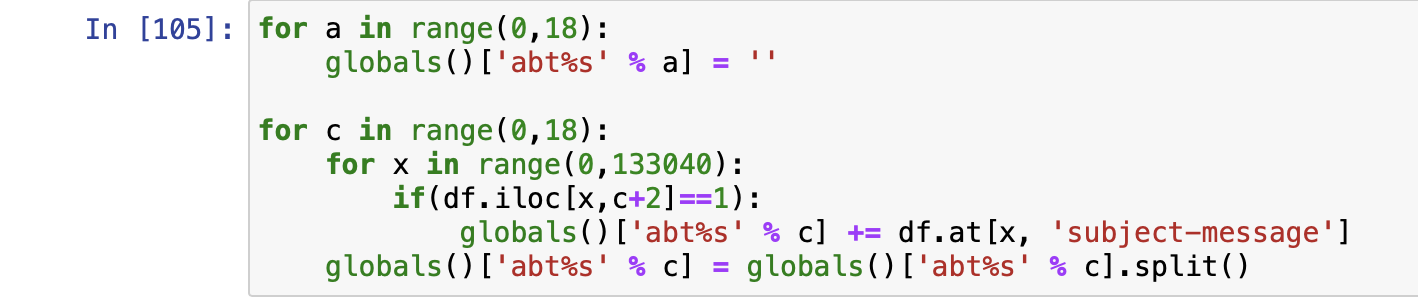
\includegraphics[scale=0.5]{lda1_1.png}

Aus dem „Wenn“-Statement ist zu erkennen, dass nur die subject-messages zum „result0“ hinzugefügt werden, die in der Tabelle bei Abteilung 0 eine 1 haben. Das Ergebnis wird dann direkt in einzelne Listenelemente unterteilt, damit ein Dictionary erstellt werden kann.
Für jede Abteilung wird dann, wie oben bereits durchgeführt, ein Korpus generiert und dessen durchschnittliche Verteilung errechnet: 

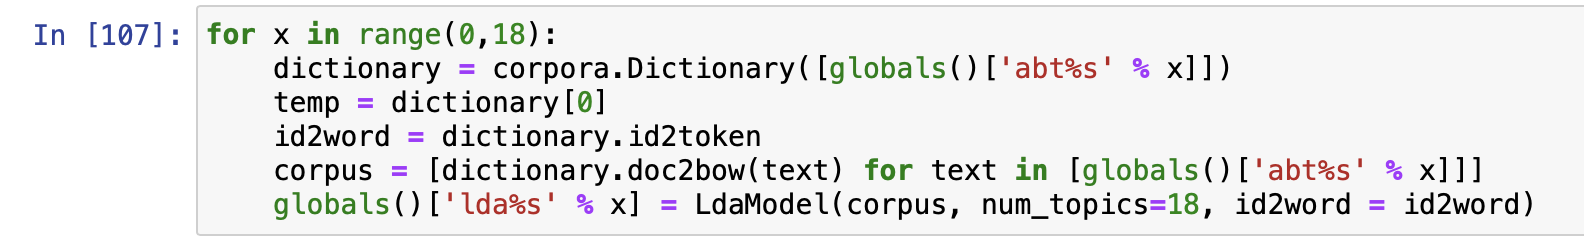
\includegraphics[scale=0.5]{lda1_2.png}

Wenn die Verteilung der Themen des Korpus gegeben ist, kann nun ein neues Dokument in diesen Korpus integriert werden und auf Basis der Wort-Themenverteilung eine Dokument-Themenverteilung des unbekannten Dokuments errechnet werden. 


\textcolor{red}{Ein unbekanntes Dokument muss mit jeder Abteilung verglichen werden. Wie mache ich das?}


\begin{comment}
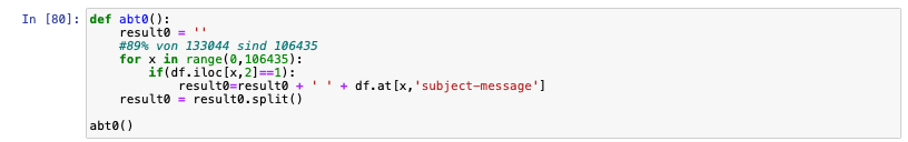
\includegraphics[scale=0.5]{lda1_3.png} --der 80% Versuch

Für diesen Korpus wird nun ein LDA Modell generiert, wie folgt: 

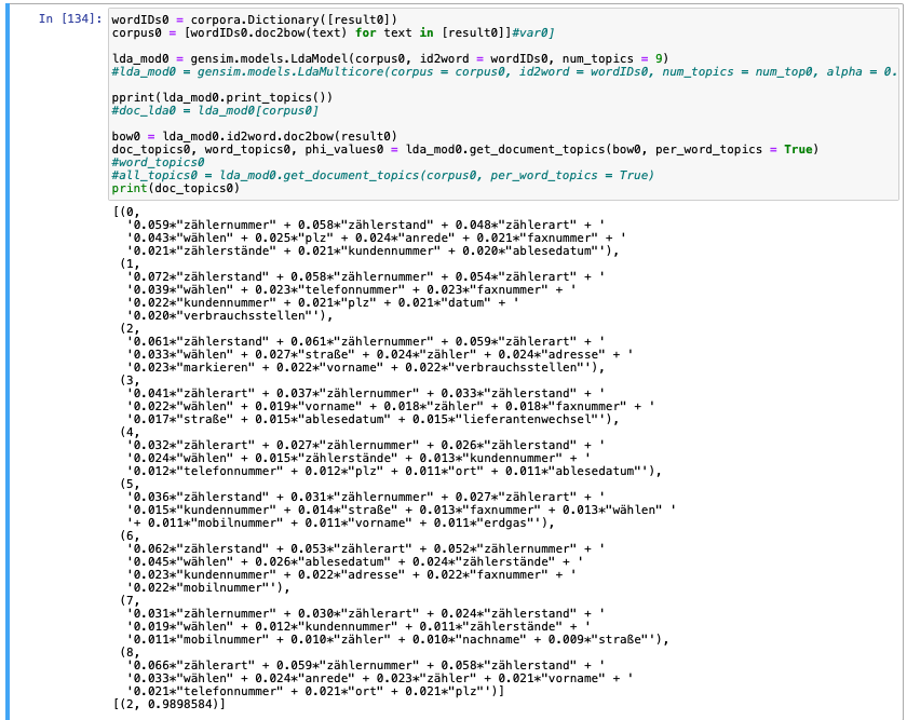
\includegraphics[scale=0.5]{lda1_4.png}

Aus den verbleibenden 20\% wird nun eine Anfrage gewählt, von der bekannt ist, dass sie der 1. Abteilung zugeordnet wurde. In diesem Fall ist das Zeile 133007. Diese wird in einen neuen Korpus verwandelt. \textcolor{red}{Muss für das Dokument wirklich ein neuer Korpus gemacht werden, um dann die Verteilungen vergleichen zu können oder kann man das Dokument auch anders in den Korpus inferieren?}

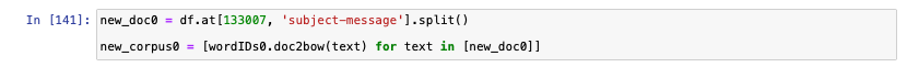
\includegraphics[scale=0.5]{lda1_5.png}

Für diesen neuen Korpus wird nun die Dokument-Themenverteilung errechnet, über der gleichen Wort-Themenverteilung. Die Ergebnisse werden dann ausgegeben und mit den des großen Korpus‘ verglichen. 

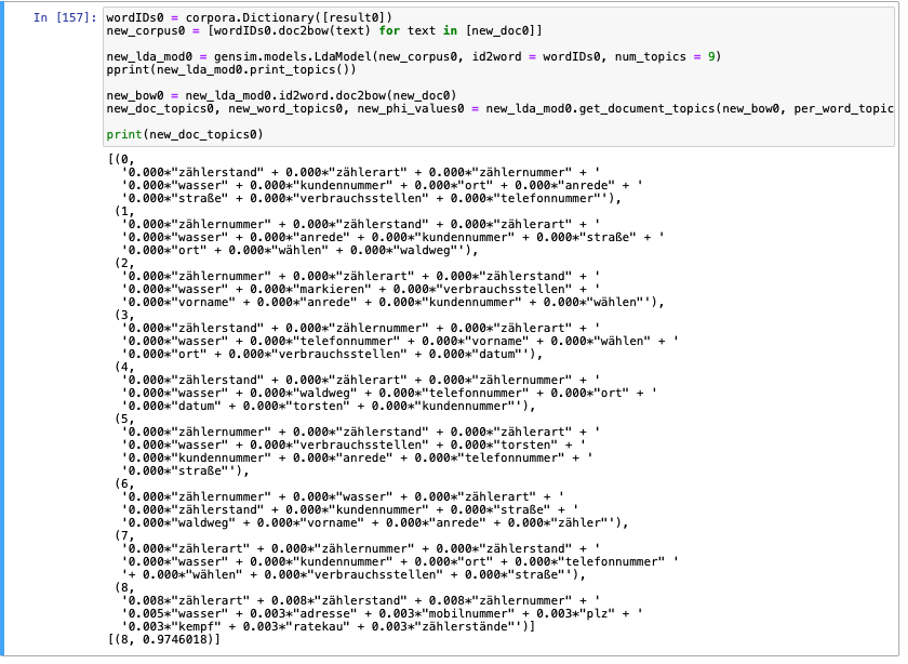
\includegraphics[scale=0.5]{lda1_6.png}
\end{comment}

\subsection{Alternativ zu Möglichkeit 1 (Erster Versuch)} Das Ziel ist die Generierung einer Themenverteilung über alle Dokumente im Korpus. Diese könnte Aufschluss über die generelle Kategorien der Abteilungen geben. Dafür müssen zuerst alle Daten in einen großen Korpus vereinigt werden, das ist in der Methode „returnAll()“ implementiert. Danach wird diese in eine Liste aufgeteilt und in ein Dictionary verwandelt. Diese wird dann genutzt um mit der „gensim.models.LdaMulticore()“-Methode in einen LDA Modell verwandelt wird. Für dieses Modell wurde die Themenanzahl auf 18 gesetzt, da dies die aktuelle Anzahl der Themen bei dem ZVO ist. 

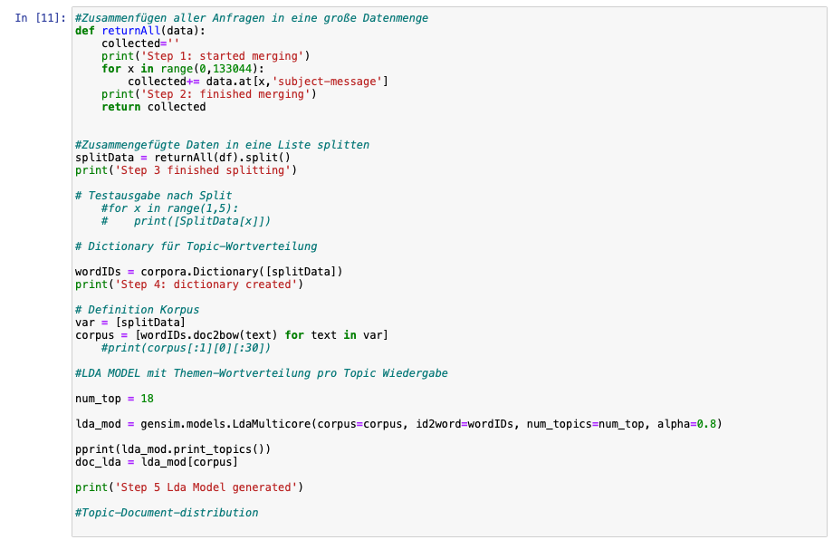
\includegraphics[scale=0.5]{lda1.png}
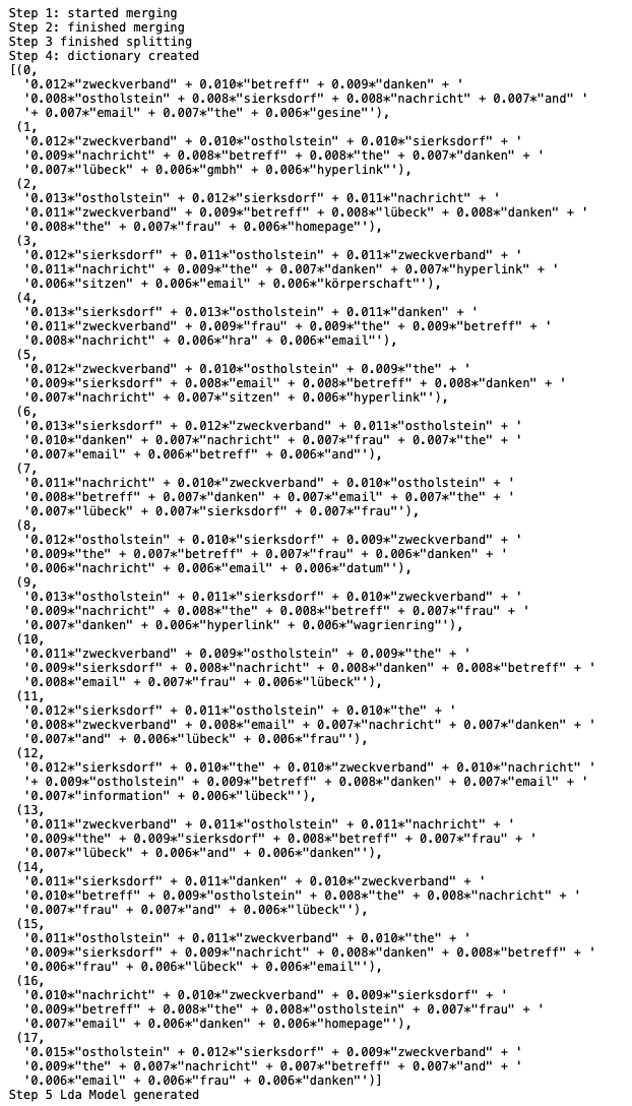
\includegraphics[scale=0.5]{lda2.png}

Der Output zeigt eine Liste mit 18 Elementen. Jedes Element beschreibt die Wortverteilung in einem der 18 Themen. Dabei kann LDA das Thema nicht semantisch benennen, sondern nur Cluster an häufig zusammen vorkommenden Wörtern formen. Daher kommt auch der „Latent“-Teil in der Benennung. Neben der Themen-Wortverteilung ist die Dokument-Themenverteilung von Interessen, also wie häufig kommt jedes Topic in der Gesamtmenge aller Anfragedaten vor. Diese Information errechnet man sich, indem man die folgende Methode aufruft:

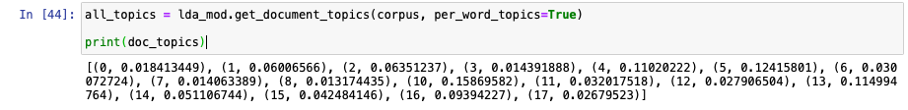
\includegraphics[scale=0.5]{lda3.png}

Aus dieser Ausgabe wird nun ersichtlich, wie wahrscheinlich es ist, dass ein bestimmtes Thema in den Daten vorkommt. Das 10. Thema ist mit 15,9\% das am häufigsten Vorkommende Thema und damit sind die Wörter „zweckverband“, „ostholstein“ und „sierksdorf“ die am stärksten vertretenen Wörter im Gesamtkorpus. Dieses Ergebnis überrascht nur bedingt, da dies der Name der Organisation ist und demensprechend häufig in Anfragen vorkommt. 

Wenn man den gleichen Quelltext mit einer geringeren Themenanzahl aufruft, kommt man auf ein ähnliches Ergebnis, hier mit Beispiel 4: 

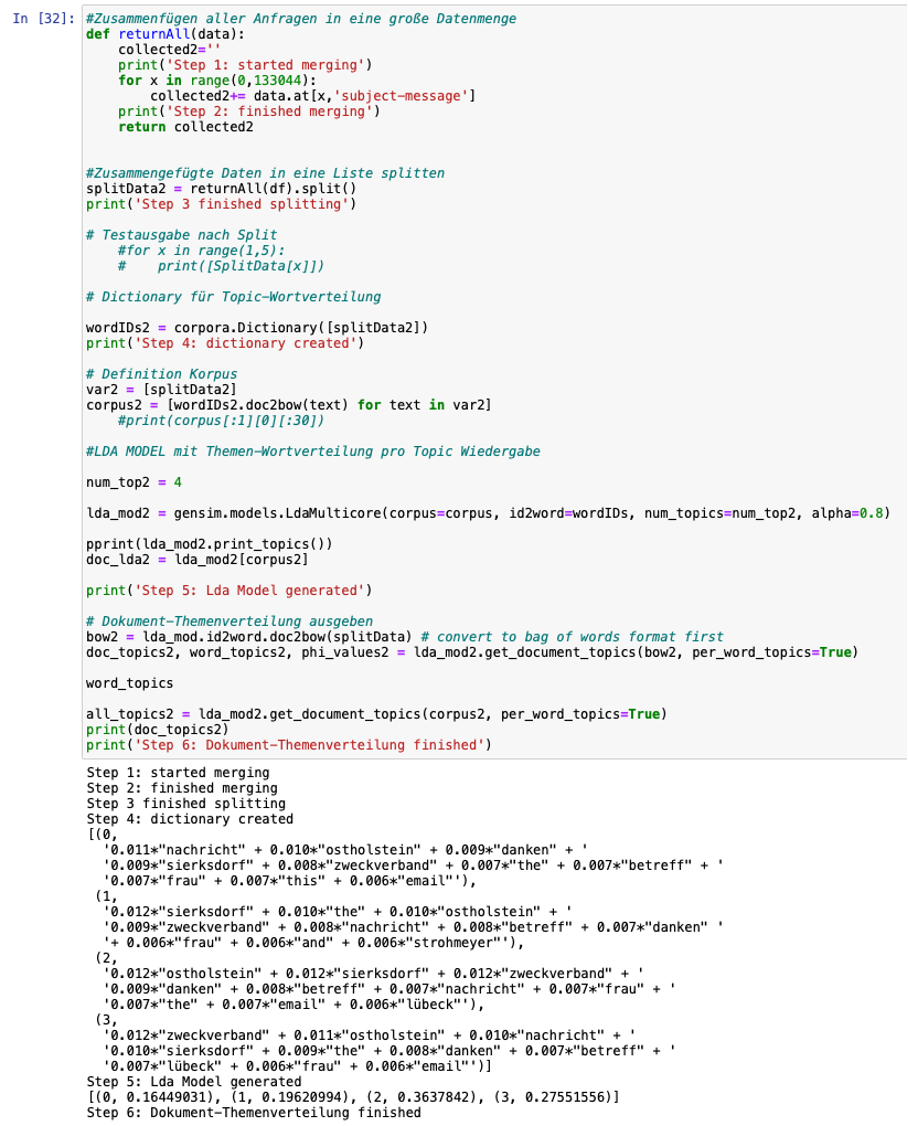
\includegraphics[scale=0.5]{lda4.png}

Wieder hat das meistvertrene Thema die Wörter „Zweckverband“, „sierksdorf“ und „ostholstein“ als häufigste vorkommende Elemente. Als Einflussfaktor dient die Dirichlet Variable Alpha, die beeinflusst, wie stark die Wahrscheinlichkeitsunterschiede zwischen den einzelnen Werten ist. Im vorherigen Beispiel war Alpha 0,8 von 1.0. Im folgenden ist es 0,2 von 1.0: 

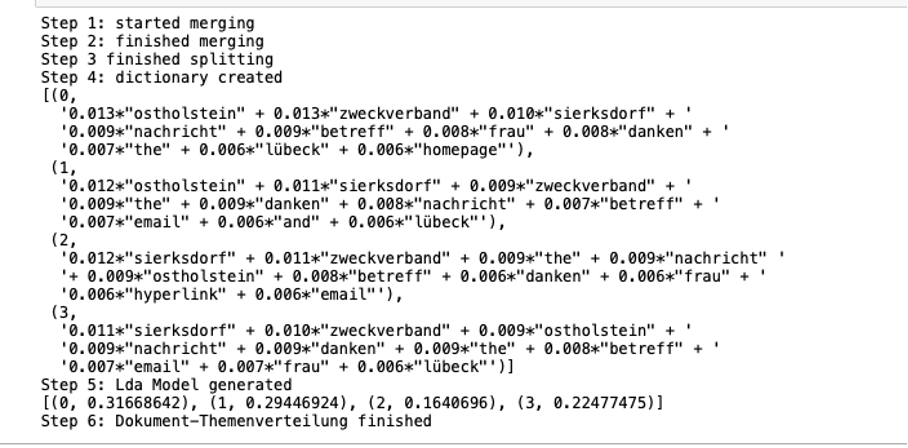
\includegraphics[scale=0.5]{lda5.png}

\textcolor{red}{Was bringt mir das?}

\subsection{\textcolor{red}{Möglichkeit 3 ??}}

\section{Auswertung}
	\subsection{Quellcode}
	\subsection{Perplexität}
	\subsection{ZVO}

	

\chapter{Conclusion}
% In a German thesis write: \subsection{Zusammenfassung und Ausblick}


% !!!!!!!!!!!!!!!!!!!!!!!!!!!!!!!!!!
% !!! Your action is needed here !!!
% !!!!!!!!!!!!!!!!!!!!!!!!!!!!!!!!!!
%
% Replace the following with your conclusion



...



% Normally, the bibliography comes next at this point. Do *not* (try
% to) include further indices and tables like an index or
% a list of figures or a list of tables or such things. Nobody
% actually uses them and they just use up space. 
%
% You *can* however include a glossary, if this seems appropriate. It
% goes here as an unnumbered chapter. Most thesis will *not* need a
% glossary: a well-written text (re)explains strange words and
% concepts as necessary. However, there are situations where a
% glossary may be helpful.














%%%
% 
% Bibliographies
%
%%%
%
% The uzl-thesis class will load biblatex for the bibliography
% management. This is a powerful package, see its documentation for
% details. The styles will be setup correctly and automatically by
% choosing one of the two style keys as described earlier.
%
% In order for the bibliography to work, run latex in the following
% order (which is the standard order):
% 
% > lualatex thesis-example
% > bibtex thesis-example
% > lualatex thesis-example
% 
% Add BibTeX files using \addbibresource or use the {bibtex entries}
% environment (see below).
%
%%%
%
% Although everyting is normally setup automatically, you can change
% the options passed to biblatex using the key 'biblatex';
% for instance,
%
%   \UzLThesisSetup{biblatex={firstinits=false}}
%
% will switch off shortened first names. Normally, you will not need
% this key in your preamble. 
% 
% Note that the bibtex program is used as the 'backend' of biblatex
% by default (rather than biber, which is the preferred program of
% biblatex). This means that you can (and must) run *bibtex* after you
% have run lualatex on your thesis. If you wish to use biber instead
% of bibtex, say 'biblatex={backend=biber}'. 
% 
%%%
%
% The following environment is optional. It allows you to keep the
% bibtex entries for your thesis right here in the thesis file. What
% happens is that each time this tex file is processed, the contents
% of the following environment gets written to the file
% \jobname-bibtex-entries.bib (this file gets overwritten each
% time). Independently, \addbibresource{\jobname-bibtex-entries.bib}
% is always called if the file \jobname-bibtex-entries.bib
% exists. 
%
% In result, you can edit and keep the bibliography's bibtex entries
% right here. If you change something here, run latex, then bibtex,
% then latex once more.
%
% If you would like to manage the bibtex entries in a separate file,
% remove the below environment, delete the \jobname-bibtex-entries.bib
% file and instead write
%
% \addbibresource{filename-of-your-bibtex-file.bib}
%
% in the preamble.
%
%%%


% !!!!!!!!!!!!!!!!!!!!!!!!!!!!!!!!!!
% !!! Your action is needed here !!!
% !!!!!!!!!!!!!!!!!!!!!!!!!!!!!!!!!!
%
% Replace following example entries with the ones of your thesis.

\begin{bibtex-entries}

@Book{Knuth1986,
  author =       {Donald Erwin Knuth},
  title =        {The \TeX book},
  publisher =    {Addison-Wesley},
  year =         {1986},
}

@Book{Lamport1994,
  author =       {Leslie Lamport},
  title =        {\LaTeX: A Document Preparation System},
  publisher =    {Addison-Wesley},
  edition =      {Second edition},
  year =         {1994},
}

@TechReport{Kernighan1974,
  author =       {Brian Kernighan},
  title =        {Programming in C – A Tutorial},
  institution =  {Bell Laboratories},
  year =         {1974}
}

@Manual{Tantau2019,
  author =       {Till Tantau},
  title =        {The Ti\emph kZ and PGF Packages: Manual for version 3.1.3},
  institution =  {Institut für Theoretische Informatik, Universität zu Lübeck},
  year =         {2019},
  url =          {https://github.com/pgf-tikz/pgf}
}

@Book{Alley1996,
  author =       {Michael Alley},
  title =        {The Craft of Scientific Writing},
  publisher =    {Springer},
  year =         {1996},
  edition =      {Third Edition},
}

@Book{DowneyF13,
  author =       {R. G. Downey and M. R. Fellows},
  title =        {Fundamentals of Parameterized Complexity},
  series =       {Texts in Computer Science},
  publisher =    {Springer},
  year =         2013,
  doi =          {10.1007/978-1-4471-5559-1},
}

@Manual{biblatex,
  title =        {The \textsc{BibLaTeX} package},
  subtitle =     {Sophisticated Bibliographies in \LaTeX},
  author =       {Kime, Philip and Lehman, Philipp},
  url =          {https://github.com/plk/biblatex},
  urldate =      {2019-06-11},
  date =         {2018-10-30},
  version =      {3.12}
}

@Manual{varioref,
  title =        {The \textsc{varioref} package},
  subtitle =     {Intelligent page references},
  author =       {Mittelbach, Frank},
  url =          {http://www.ctan.org/pkg/varioref},
  urldate =      {2019-06-11},
  date =         {2016-02-16},
  version =      {1.5c}
}

@Manual{hyperref,
  title =        {The \textsc{hyperref} package},
  subtitle =     {Extensive support for hypertext in \LaTeX},
  author =       {Rahtz, Sebastian and Oberdiek, Heiko},
  url =          {https://github.com/ho-tex/hyperref},
  urldate =      {2019-06-11},
  date =         {2018-11-30},
  version =      {6.88e}
}

@Manual{babel,
  title =        {The \textsc{babel} package},
  subtitle =     {Multilingual support for Plain \TeX\ or \LaTeX},
  author =       {Braams, Johannes L. and Bezos López, Javier},
  url =          {http://www.ctan.org/pkg/babel},
  urldate =      {2019-06-11},
  date =         {2019-06-03},
  version =      {3.32}
}

@Manual{fontspec,
  title =        {The \textsc{fontspec} package},
  subtitle =     {Advanced font selection in Xe\LaTeX\ and Lua\LaTeX},
  author =       {Robertson, Will},
  url =          {http://www.ctan.org/pkg/fontspec},
  urldate =      {2019-06-11},
  version =      {2.7c}
}

@Manual{url,
  title =        {The \textsc{url} package},
  subtitle =     {Verbatim with \textsc{url}-sensitive line breaks},
  author =       {Arseneau, Donald},
  url =          {http://www.ctan.org/pkg/url},
  urldate =      {2019-06-11},
  date =         {2013-09-16},
  version =      {3.4}
}

@Manual{amsmath,
  title =        {The \textsc{amsmath} package},
  subtitle =     {\AmS\ mathematical facilities for \LaTeX},
  author =       {{The \LaTeX\ Team}},
  url =          {http://www.ams.org/tex/amslatex.html},
  urldate =      {2019-06-11}, 
  date =         {2017-09-02},
  version =      {2.17a}
}

@Book{Beutelspacher2009,
  title =        {„Das ist o.\,B.\,d.\,A.\ trivial!“: Tipps und Tricks zur
                  Formulierung mathematischer Gedanken (Mathematik für
                  Studienanfänger)},
  author =       {Albrecht Beutelspacher},
  year =         {2009},
  edition =      {Ninth, updated edition},
  publisher =    {Vieweg+Teubner Verlag},
  doi =          {10.1007/978-3-8348-9075-7},
}

\end{bibtex-entries}



% If you need to have an appendix (I advise against it), insert it
% here using, first, \appendix and then \chapter and then,
% possibly, \section. 
%
% \appendix
%
% \chapter{Technical Appendix}
%
% \section{Experimental Parameters} % possibly
%
% Again, I advise against using an appendix.


\end{document}

%  LocalWords:  LaTeX tex moretexcs Lübeck pdf uzl lualatex bibtex th
%  LocalWords:  TechReport Kernighan Lamport's Tantau's Tantau cls kZ
%  LocalWords:  Mustermann emacs oldschool pdflatex texmf utf biber
%  LocalWords:  biblatex Alphabetische Bibliographie Numerische VIIa
%  LocalWords:  varioref german Einleitung Beiträge dieser Arbeit xml
%  LocalWords:  Ergebnisse Verwandte Arbeiten Aufbau nucleotide VIIc
%  LocalWords:  ensembl amino phylogenetic Alexa Siri decrypt versa
%  LocalWords:  cryptographic pre nondeterministic deterministically
%  LocalWords:  Beutelspacher Untersuchungen zum genetischen sep llcc
%  LocalWords:  Beispiel tikz jpg png Alegrya Kasimir Malewitsch PGF
%  LocalWords:  Lamport Institut für Theoretische Informatik zu url
%  LocalWords:  Universität Springer DowneyF Downey Parameterized doi
%  LocalWords:  BibLaTeX Kime Philipp urldate Mittelbach hyperref Lua
%  LocalWords:  Rahtz Oberdiek Heiko Braams Bezos López fontspec Das
%  LocalWords:  Arseneau amsmath ist Tipps und zur Formulierung
%  LocalWords:  mathematischer Gedanken Mathematik Studienanfänger
%  LocalWords:  Albrecht Vieweg Teubner Verlag
